\section{Results}
\subsection{Controlled Visual Test and Asynchronous Integration}
The separate visual test set contained 30 photographs per class, for a total of 180 images. The images were acquired under fixed viewpoint, background, and lighting conditions and were not used for model training or parameter selection. The model correctly classified all 180 images and mapped every prediction to the intended strategy. Mean confidence was 0.853, and mean per-image inference wall-clock time was 48.19 ms (Table~\ref{tab:7} and Figs.~\ref{fig:4} and \ref{fig:5}). These results characterize the six known object instances under controlled imaging conditions. They do not quantify online trigger correctness, false-trigger/default-branch frequency, end-to-end trigger latency, or completion of configuration before contact during the 135 teleoperation trials.

\begin{table}[!t]
\centering
\caption{Class-wise results of the closed-set controlled visual test.}
\label{tab:7}
\small
\setlength{\tabcolsep}{4pt}
\renewcommand{\arraystretch}{1.16}
\begin{tabular*}{\columnwidth}{@{\extracolsep{\fill}}lccc@{}}
\toprule
Object & Images & Mean confidence & Mean time (ms) \\
\midrule
Apple & 30 & 0.771 & 49.89 \\
Banana & 30 & 0.948 & 48.02 \\
Bottle & 30 & 0.726 & 48.57 \\
Paper cup & 30 & 0.820 & 46.62 \\
Mouse & 30 & 0.914 & 46.79 \\
Scissors & 30 & 0.938 & 49.27 \\
\bottomrule
\end{tabular*}
\par\smallskip
\footnotesize\textit{Note:} All 180 images were classified correctly and mapped to the intended strategy under the fixed viewpoint, background, and lighting conditions. This table does not quantify online trigger correctness, false triggers, or trigger-to-contact timing during teleoperation.
\end{table}
\begin{figure}[!t]
\centering

\includegraphics[width=\columnwidth]{fig4.png}
\caption{Confusion matrix for the separate closed-set controlled visual test (180 images; 30 images per class). Each cell gives the number of images for the corresponding true and predicted class. All observations lie on the diagonal under the fixed viewpoint, background, and lighting conditions.}
\label{fig:4}
\end{figure}

\begin{figure*}[!t]
\centering

\includegraphics[width=\textwidth]{fig5.png}
\caption{Detection confidence and per-image inference wall-clock time for the closed-set controlled 180-image visual test ($n=30$ images per class). (a) Class-wise confidence: horizontal bars show mean $\pm$ SD; the dotted and dashed vertical lines mark the decision threshold (0.25) and overall mean (0.853). (b) Per-image processing time: half violins show class-wise distributions, dots show individual images, horizontal segments and open circles show the IQR and median, and the dashed vertical line marks the overall mean (48.19 ms). These timing data are not end-to-end task-trigger latency measurements.}
\label{fig:5}
\end{figure*}

In the supervisory-loop implementation, the independent YOLO process, bounded queues, and non-blocking polling kept visual inference outside the synchronous call path of the nominal 200-Hz update. The median logged cycle time was 5.07 ms.

\subsection{Results Across the Five Modes}
\begin{table*}[!t]
\centering
\caption{Descriptive results across the five experimental modes.}
\label{tab:8}
\small
\setlength{\tabcolsep}{5pt}
\renewcommand{\arraystretch}{1.16}
\begin{tabularx}{\textwidth}{@{}p{0.11\textwidth}YYYp{0.15\textwidth}@{}}
\toprule
Mode & Completion time (s) & Trajectory length (m) & Success rate & Raw NASA-TLX \\
\midrule
A & 21.18 [20.62, 22.08] & 0.757 [0.693, 0.816] & 22/27 (81.5\%) & 62.50 [59.67, 64.50] \\
B & 20.89 [20.12, 21.83] & 0.787 [0.721, 0.861] & 21/27 (77.8\%) & 56.17 [55.00, 59.33] \\
\textbf{C} & \textbf{19.57 [18.41, 20.05]} & \textbf{0.697 [0.660, 0.769]} & \textbf{26/27 (96.3\%)} & \textbf{48.67 [47.67, 51.83]} \\
D & 20.79 [20.32, 21.16] & 0.722 [0.678, 0.768] & 24/27 (88.9\%) & 60.33 [57.33, 62.50] \\
E & 20.73 [19.95, 22.25] & 0.732 [0.678, 0.799] & 24/27 (88.9\%) & 53.67 [51.83, 57.83] \\
\bottomrule
\end{tabularx}
\par\smallskip
\footnotesize\textit{Note:} Values are median [IQR], except success rate. Completion time, trajectory length, and success rate use $n=27$ trials per mode; Raw NASA-TLX uses $n=9$ strategy-level questionnaire units per mode. Mode definitions are given in Table~\ref{tab:3}; trial-level performance data are provided in Supplementary Table S1.
\end{table*}
Mode C had the lowest median completion time, the highest observed success rate, and the lowest Raw NASA-TLX score (Table~\ref{tab:8} and Figs.~\ref{fig:6} and \ref{fig:7}). It also had the lowest median master-side trajectory length, an exploratory measure. Using the trial-level values in Supplementary Table S1, mean completion time in mode C (19.28 $\pm$ 1.30 s) was lower than in modes A (21.42 $\pm$ 1.58 s), B (21.01 $\pm$ 1.61 s), D (20.91 $\pm$ 1.10 s), and E (21.07 $\pm$ 1.56 s) by 10.0\%, 8.2\%, 7.8\%, and 8.5\%, respectively. Subsequent inferential analyses focused on completion time as the primary endpoint.

Consistent with the descriptive results, the Friedman test across the 27 matched task blocks indicated differences in completion time among the five modes ($\chi^2(4)=30.904$, $p<0.001$). Holm-adjusted paired Wilcoxon tests showed lower completion times in mode C than in modes A, B, D, and E (all $p<0.01$). Because the task blocks were nested within only three operators, these statistics describe repeated-measures differences within the present sample and do not support population-level inference across operators. Descriptively, mode C had the lowest Raw NASA-TLX score in all nine operator $\times$ strategy units; given the three-operator sample, no population-level workload inference was made.

\begin{figure}[!t]
\centering

\includegraphics[width=\columnwidth]{fig6.png}
\caption{Task execution duration across the five experimental modes: fixed-parameter baseline (A), manual-selection workflow baseline (B), joint parameter-bundle configuration (C), visual-semantic display with fixed parameters (D), and impedance-only reconfiguration (E). Each mode contains 27 matched task blocks. Filled circles show medians, thick horizontal segments show IQRs, thin horizontal segments with end caps show 1.5 $\times$ IQR Tukey whiskers, and small open circles show observations beyond the whiskers. This descriptive distribution plot does not display the block pairing; the primary C--E pairing is shown in Fig.~\ref{fig:8}.}
\label{fig:6}
\end{figure}

\begin{figure*}[!t]
\centering

\includegraphics[width=\textwidth]{fig7.png}
\caption{Human workload and observed task success across the five experimental modes. (a) Raw NASA-TLX scores: connected markers show each operator's mean across three strategy-level questionnaire units per mode ($n=9$ questionnaire units per mode); marker shape identifies the operator. (b) Observed successful trials out of 27 for each mode. These panels are descriptive and do not display confidence intervals or inferential tests.}
\label{fig:7}
\end{figure*}

\subsection{Primary Comparison: Complete Parameter Bundle Versus Impedance-Only Reconfiguration}
Table~\ref{tab:9} summarizes the primary C--E comparison.

\begin{table*}[!t]
\centering
\caption{Within-sample primary comparison of the complete parameter bundle and impedance-only reconfiguration.}
\label{tab:9}
\small
\setlength{\tabcolsep}{5pt}
\renewcommand{\arraystretch}{1.16}
\begin{tabularx}{\textwidth}{@{}p{0.18\textwidth}YYYp{0.20\textwidth}@{}}
\toprule
Measure & C, median [IQR] & E, median [IQR] & Mean $\Delta$ (E--C), 95\% CI & Operator direction \\
\midrule
Completion time (s) & 19.57 [18.41, 20.05] & 20.73 [19.95, 22.25] & 1.79 [1.10, 2.51] & 3/3 favored C \\
Trajectory length (m) & 0.697 [0.660, 0.769] & 0.732 [0.678, 0.799] & 0.024 [-0.014, 0.059] & Mixed \\
Raw NASA-TLX & 48.67 [47.67, 51.83] & 53.67 [51.83, 57.83] & 4.87 [not calculated] & 3/3 favored C \\
\bottomrule
\end{tabularx}
\par\smallskip
\footnotesize\textit{Note:} Positive $\Delta$ values favor mode C. Completion time and trajectory length use $n=27$ matched task blocks; Raw NASA-TLX uses $n=9$ questionnaire units per mode. Intervals are matched-task-block bootstrap 95\% CIs from 10,000 resamples and quantify uncertainty across the observed blocks, not a population-level participant effect; no bootstrap interval was calculated for Raw NASA-TLX.
\end{table*}
The median completion times were 19.57 s in mode C and 20.73 s in mode E (Fig.~\ref{fig:8}). With $\Delta T=T_E-T_C$, the mean paired difference was 1.79 s and the bootstrap 95\% CI was [1.10, 2.51] s, corresponding to a mean reduction of 8.5\%. Completion time was lower in mode C in 22 of the 27 matched blocks. The mean differences for P01, P02, and P03 were 1.66, 2.56, and 1.16 s, respectively. Across the six objects, the relative differences ranged from 3.3\% to 13.2\% (Fig.~\ref{fig:9}).

As a post hoc sensitivity analysis, the C--E completion-time comparison was repeated after retaining only the 23 matched blocks in which both trials were successful. The mean paired difference remained 1.80 s, and 19 of the 23 blocks favored mode C. This descriptive sensitivity result indicates that the primary mean difference was not driven by the four blocks with a failure in either mode.

For paired success outcomes, 23 blocks succeeded in both modes, three succeeded in mode C and failed in mode E, one failed in mode C and succeeded in mode E, and none failed in both modes. With only four discordant pairs, the exact two-sided McNemar test did not establish a difference ($p=0.625$). The observed success-rate difference is therefore interpreted as supplementary descriptive evidence rather than as a confirmed mode effect.

The median master-side trajectory lengths were 0.697 m in mode C and 0.732 m in mode E. The mean paired difference was 0.024 m, with a bootstrap 95\% CI of [-0.014, 0.059] m. Pause counts were lower on average in mode C but had the same median in modes C and E.

\begin{figure}[!t]
\centering

\includegraphics[width=\columnwidth]{fig8.png}
\caption{Paired completion-time comparison between modes C and E for 27 matched task blocks across three operators. (a) Each point represents one matched block; points below the identity line have a shorter duration in mode C. (b) Distribution of the paired difference $\Delta T=T_E-T_C$; positive values favor mode C. The violin, horizontal segment, and diamond show the distribution, median, and mean, respectively. The observed mean difference was 1.79 s (matched-block bootstrap 95\% CI, 1.10--2.51 s), and 22/27 blocks favored C; the interval is conditional on the observed blocks.}
\label{fig:8}
\end{figure}

\subsection{Exploratory Process Measure: C--E Pause Analysis}
Pause count was analyzed as an exploratory process measure using master-side trajectories sampled at approximately 200 Hz. A pause was defined as a continuous interval in which master-device speed remained below 0.005 m/s for at least 0.30 s, excluding momentary decelerations and capturing more sustained interruptions. Mode C had a median pause count of 3 [2, 3.5] and a mean of 2.74 $\pm$ 1.23, whereas mode E had a median of 3 and a mean of 3.41 $\pm$ 1.67. Although mode C had a lower mean in each strategy class, the two modes had the same overall median. No formal hypothesis test was prespecified or performed for pause count, and no threshold-sensitivity analysis was available.

\subsection{Failure Analysis}
Eighteen failures occurred across the 135 trials: 5, 6, 1, 3, and 3 in modes A--E, respectively. The failures included object drops, observable slip, and visible damage, as summarized in Table~\ref{tab:10}. One designated researcher recorded outcomes in real time using the predefined criteria in Section 3.4; no systematic video recording or independent re-rating was available.

\begin{table*}[!t]
\centering
\caption{Observed failures and representative observations by experimental mode.}
\label{tab:10}
\small
\setlength{\tabcolsep}{6pt}
\renewcommand{\arraystretch}{1.16}
\begin{tabularx}{\textwidth}{@{}p{0.19\textwidth}p{0.14\textwidth}Y@{}}
\toprule
Mode & Failures/total & Representative observations \\
\midrule
A & 5/27 & Paper-cup deformation and unstable positioning of the scissors. \\
B & 6/27 & The manual-selection workflow included additional judgment and switching steps; the available records do not support attribution of specific failure causes. \\
\textbf{C} & \textbf{1/27} & Mouse slip during transfer. \\
D & 3/27 & Object drops or loss of grasp during holding. \\
E & 3/27 & Observed instability during grasp establishment or transfer. \\
\bottomrule
\end{tabularx}
\par\smallskip
\footnotesize\textit{Note:} Mode definitions are given in Table~\ref{tab:3}. Observations are descriptive and were recorded in real time.
\end{table*}
Mode C had one failure in 27 trials, the lowest observed count among the five modes under the present experimental conditions.

\subsection{Consistency Across Operators and Objects}
Figure~\ref{fig:9} reports paired C--E differences by operator and object. At the operator level, the mean paired differences $\Delta T=T_E-T_C$ for P01, P02, and P03 were 1.66, 2.56, and 1.16 s, respectively. The corresponding median [IQR] differences were 1.91 [0.60, 3.14], 2.63 [2.19, 3.34], and 1.60 [-0.53, 1.73] s. Mode C was faster in 7/9, 9/9, and 6/9 task blocks, respectively. After P01, P02, and P03 were excluded in turn, the mean differences in the remaining blocks were 1.86, 1.41, and 2.11 s, respectively; all continued to favor mode C.

At the object level, mode C also had the shortest mean completion time among the five modes for each of the six objects (Table~\ref{tab:11}):

\begin{table}[!t]
\centering
\caption{Mean completion time by object and experimental mode.}
\label{tab:11}
\small
\setlength{\tabcolsep}{4pt}
\renewcommand{\arraystretch}{1.16}
\begin{tabular}{@{}lccccc@{}}
\toprule
Object & A & B & \textbf{C} & D & E \\
\midrule
Apple & 20.46 & 21.40 & \textbf{19.25} & 20.81 & 20.94 \\
Banana & 20.07 & 20.85 & \textbf{19.49} & 21.06 & 20.64 \\
Paper cup & 22.36 & 20.27 & \textbf{18.69} & 20.38 & 21.17 \\
Bottle & 22.11 & 22.14 & \textbf{19.63} & 20.78 & 20.30 \\
Mouse & 21.74 & 20.93 & \textbf{19.75} & 20.74 & 21.64 \\
Scissors & 21.79 & 20.70 & \textbf{18.84} & 21.83 & 21.70 \\
\bottomrule
\end{tabular}
\par\smallskip
\footnotesize\textit{Note:} Values are mean completion time in seconds. Mode definitions are given in Table~\ref{tab:3}; bold indicates the lowest mean in each row.
\end{table}
Relative to mode E, the mean completion-time reductions in mode C were 3.3\% for the bottle, 5.5\% for the banana, 8.1\% for the apple, 8.7\% for the mouse, 11.7\% for the paper cup, and 13.2\% for the scissors. The direction was consistent across all objects, although the magnitude varied.

\begin{figure*}[!t]
\centering
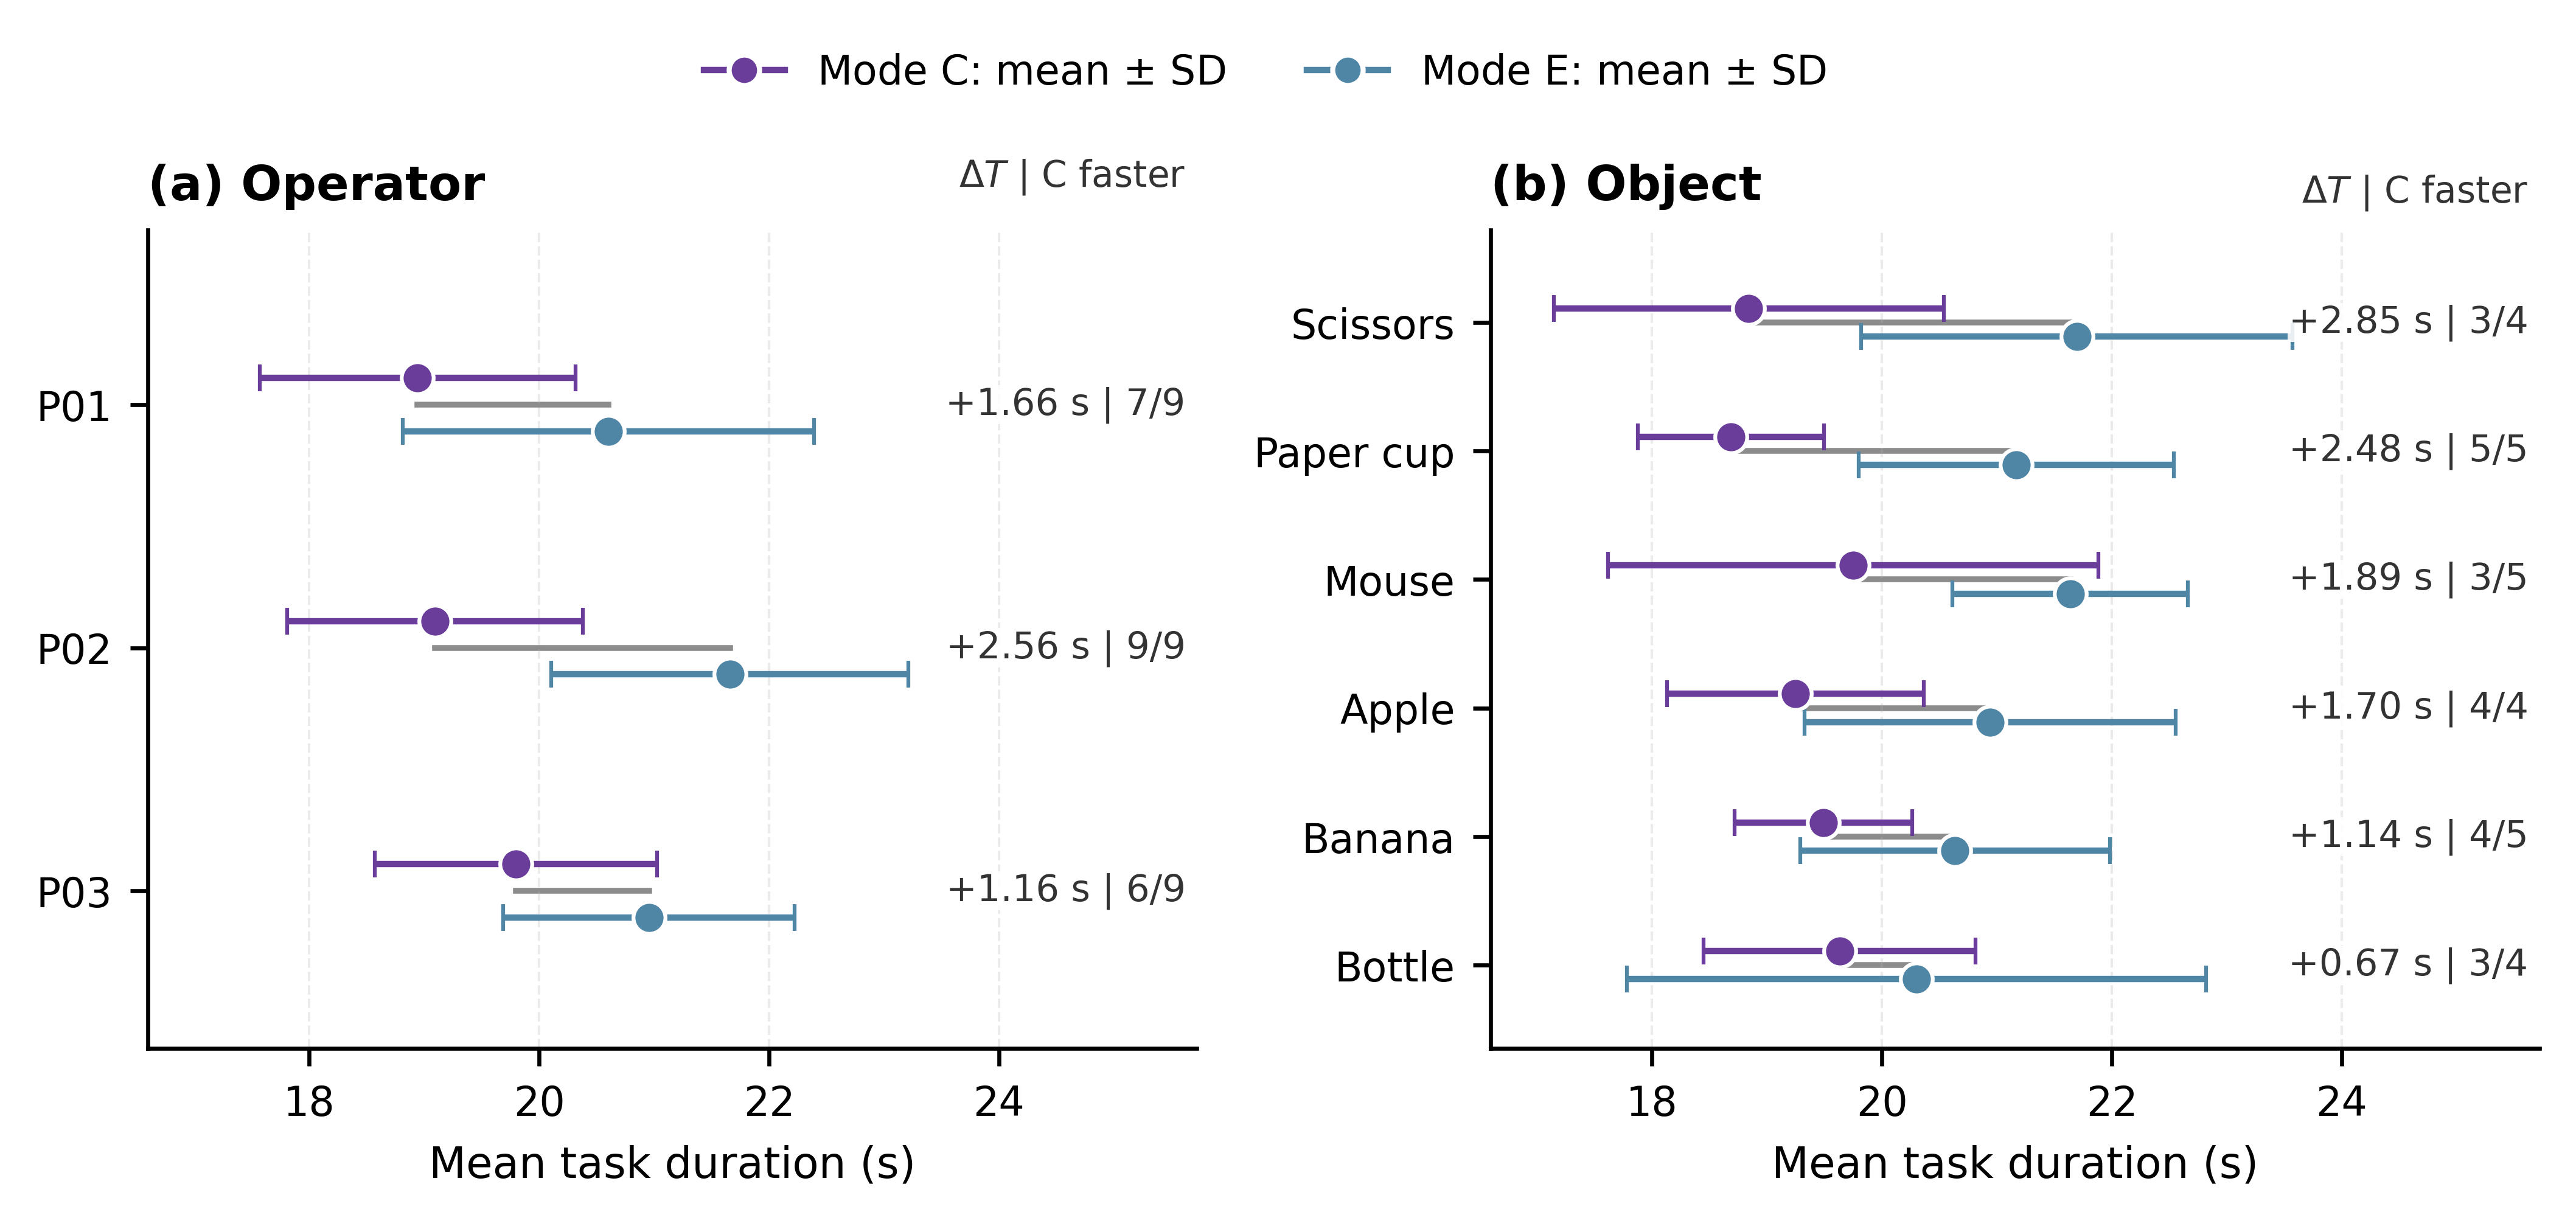
\includegraphics[width=\textwidth]{fig9.png}
\caption{Descriptive mean task duration for modes C and E, stratified by operator and object. Purple and blue points show mean $\pm$ SD for modes C and E, respectively; gray connectors link the paired means. Labels report $\Delta T=T_E-T_C$ and the number of matched blocks favoring mode C (nine per operator and four or five per object). The object-level summaries are descriptive because each contains only four or five blocks.}
\label{fig:9}
\end{figure*}
